\chapter{Introduction}
\label{chap:introduction}
\section{Biomedical and anatomic principles}
\subsection{Bilateria lineage}
Cerebral bilateral symmetry is a universal quality of organisms belonging to the Bilateria lineage \cite{Concha2012,Corballis2009}, the phylum incorporating all species with a single plane of symmetry, in contrast with their sister group, Cnidaria (\autoref{fig:bilateriaphylum}). Bilateral symmetry is a byproduct of the activity of two separate developmental processes, that produce two axes of polarity \cite{Finnerty2003}, and therefore a symmetry plane; the formation of a primary body axis, that corresponds to the long anatomical dimension of the animal, called \acf{rc} (i.e. head-to-tail), primarily dictated by highly conserved controlled activation of HOX genes during cell differentiation; the shaping of a secondary body axis, orthogonal to \ac{rc}, named \acf{dv} (i.e. back-to-front), attributed to a variety of genes,  such as the chromatin organizer CTCF, the left-right determination factor Nodal and central HOX genes \cite{Heger2020}. The remaining axis, \acf{lr}, is the one along which the symmetry pattern is manifested. On account of the high biodiversity that bilateria group includes, only the subgroup of vertebrates is examined in the following literature study. In addition, any reference to symmetry or asymmetry from now on corresponds to the \ac{lr} direction, unless explicitly mentioned.

This study makes an effort to statistically identify the genetic origins of a complex structural phenotype. Hence, examining, based on existing research, the main brain developmental stages is essential to discern the processes that induce bilateral symmetry. An important vertebrates (and bilateria) common characteristic is the germ line \textbf{triploblasticity}: the embryo begins as a flat disk, through a process called \textbf{gastrulation}, with three distinct cell layers; \textbf{endoderm}, \textbf{mesoderm}, and \textbf{ectoderm} \cite{F.Bear2016a}.  Of significance in the neural system formation is the ectoderm, which is initially equivalent to one of the flat disk sides. Under the context of this study, although a fact not directly connected to the brain cortex, it is necessary to mention that the perfect bilateral symmetry pattern appears to break even before gastrulation. In Xenopus (frog species) embryos, during fertilization and the initial 4-cell cleavage of the fertilized egg , the \textbf{cytoskeleton microtubules} appear to asymmetrically localize the ion channels proteins, whose \acs{rna} has been passed on by the mother, with a preference for the right side of the complex \cite{Aw2008}. Chicks embryos also exhibit a similar pattern. The occurrence of asymmetry at this extremely early time point underlines the significant role it has on the embryo development, species fitness, and, concomitantly, the conservation potential of this trait drivers \cite{Aw2009}. Another cellular component that is considered to enhance asymmetry, during gastrulation, is the motile cilia, hair-like organelles on the cell surface with the ability to beat \cite{Grimes2017}. Their movement is by construction asymmetric, causing a leftward flow of extraembryonic fluid and, subsequently, asymmetric distribution of exogenously introduced proteins \cite{Okada2005}. Both studied phenomena point to early initiation of asymmetric genes expression.

\begin{figure}[H]
	\centering
	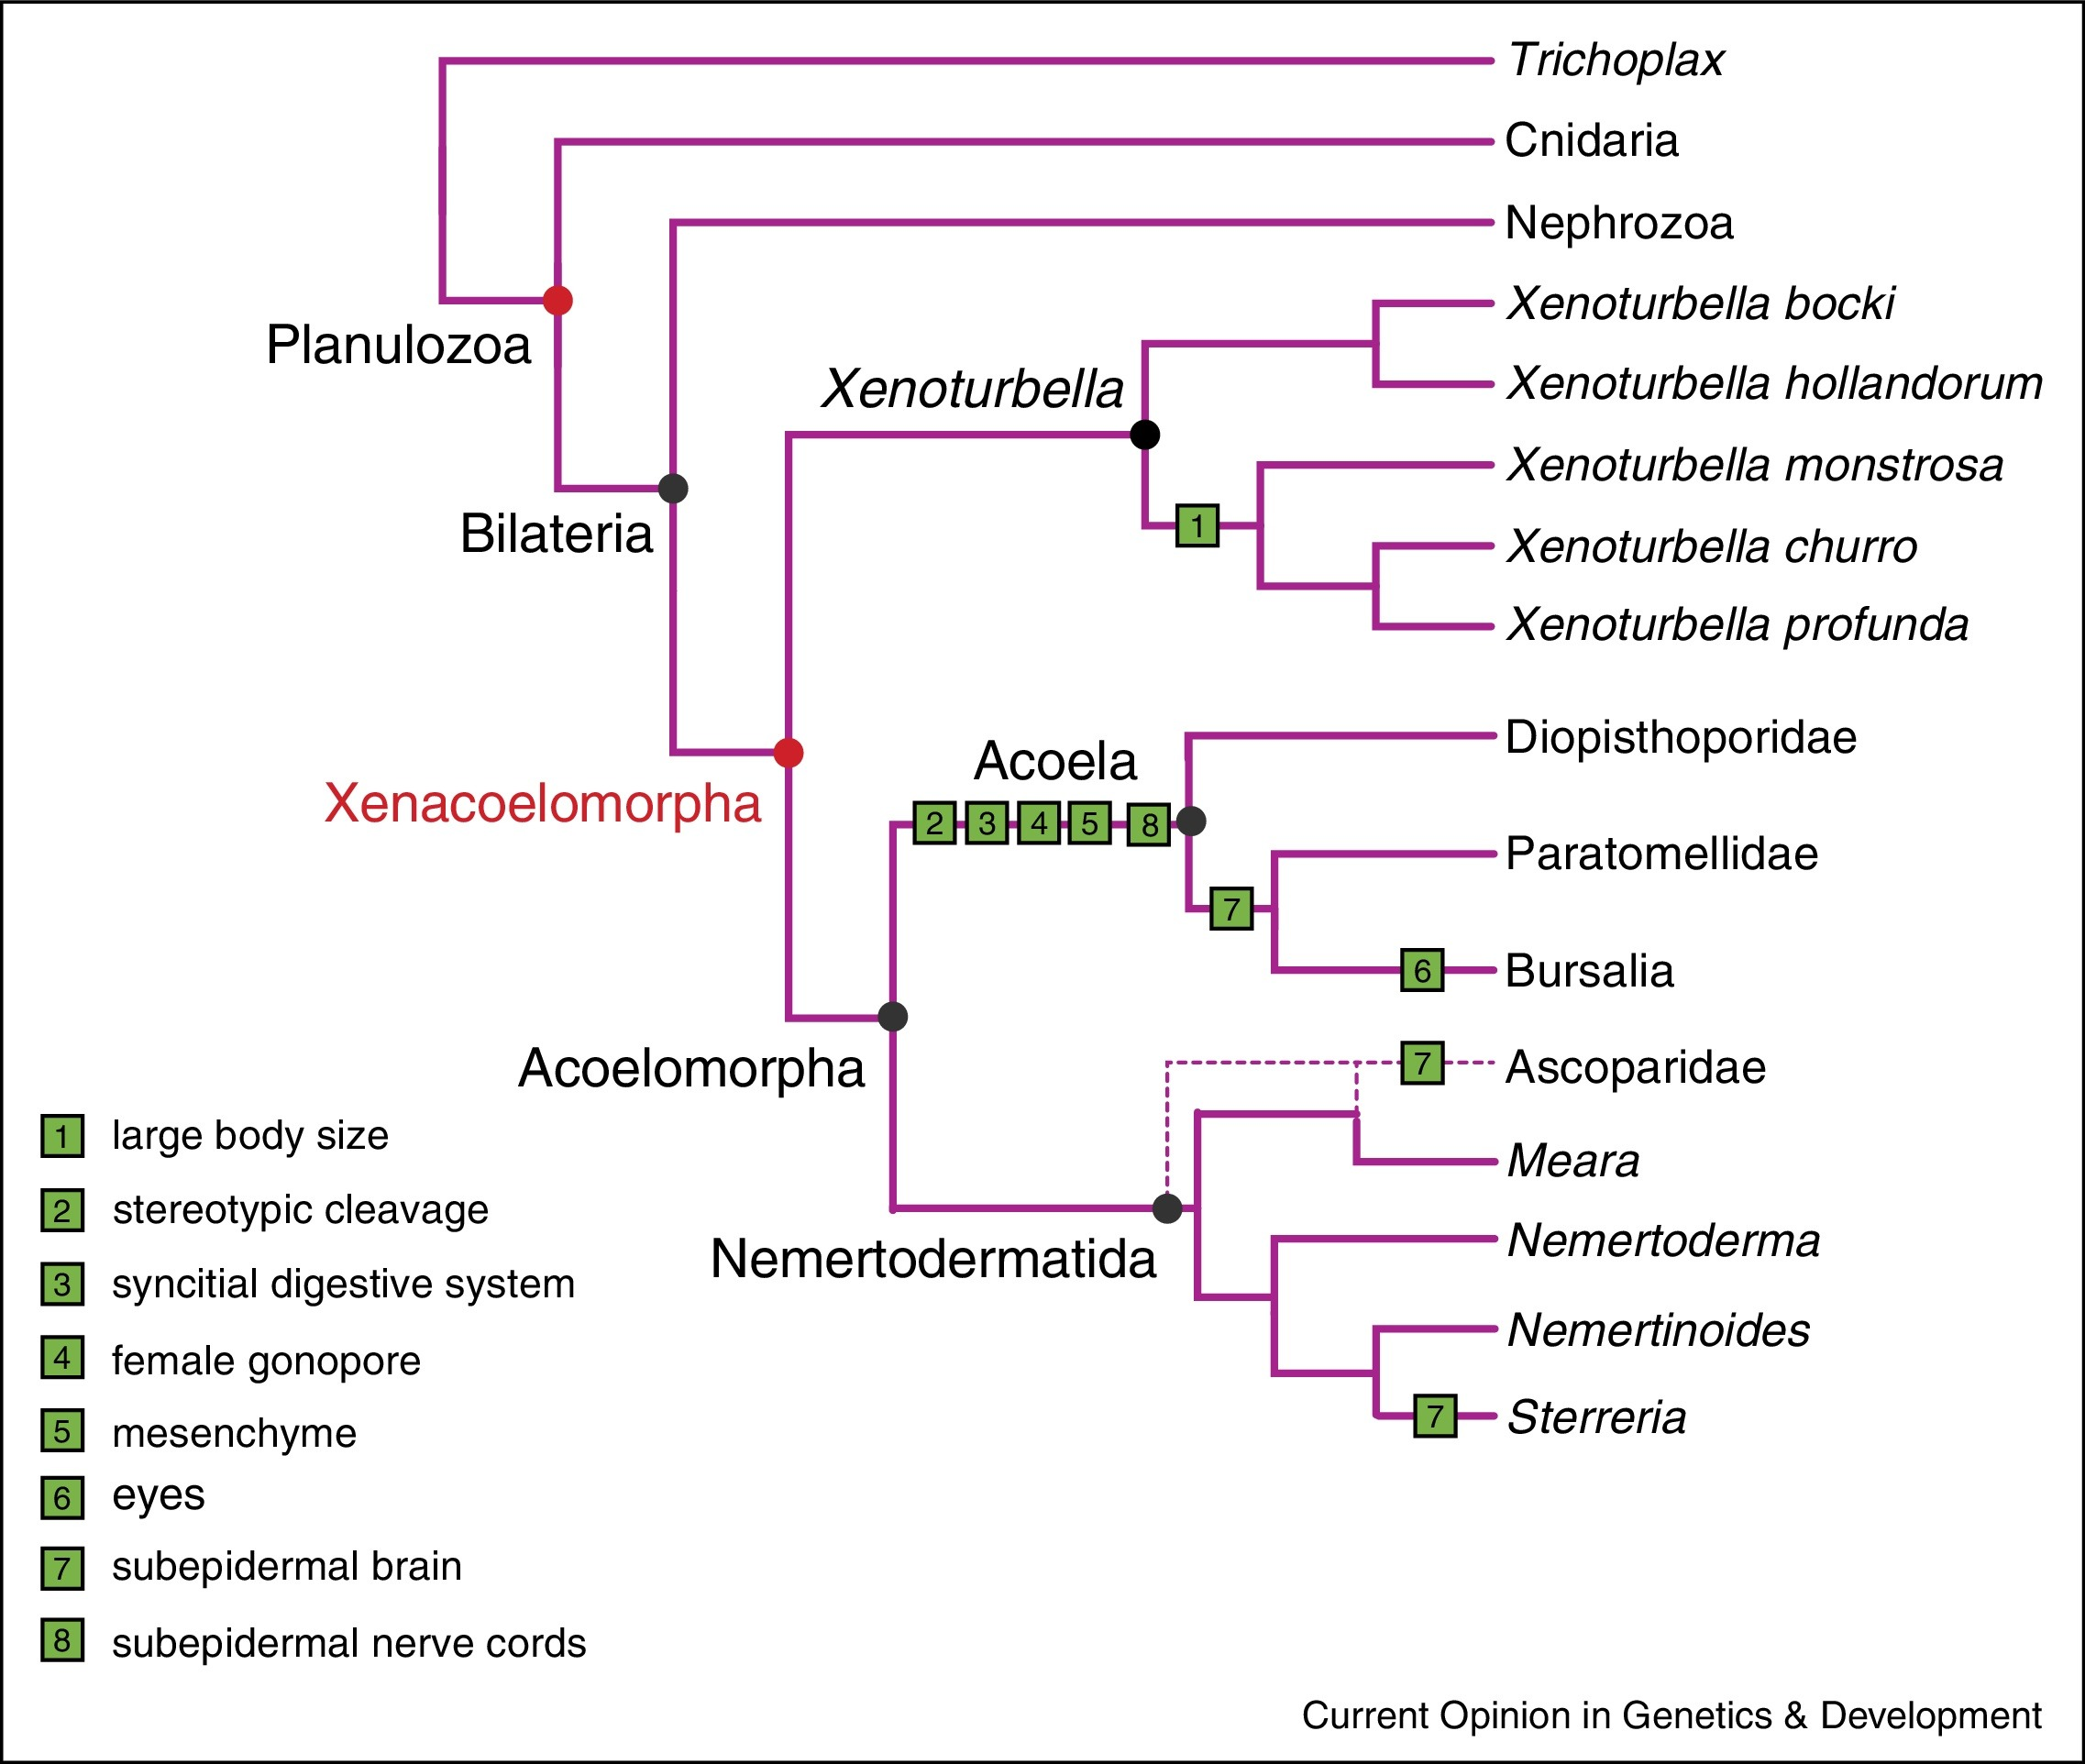
\includegraphics[width=0.9\linewidth]{bilateria_phylum}
	\caption[Bilateria clade \cite{Hejnol2016}]{Species phylogenetic tree subset, displaying bilateria clade, its sister clade, Cnidaria, and the direct children\cite{Hejnol2016}. Of great importance on the evolutionary studies of bilateral symmetry is the Xenacoelomorpha clade.}
	\label{fig:bilateriaphylum}
\end{figure}

\subsection{Symmetry during \acs{cns} formation}
Shortly after gastrulation, the disk folds, in a way that the central region of the ectoderm, called neural plate, forms a tube-like shape, the \textbf{neural tube}, which acts as the neural system precursor, under a process called \textbf{neurulation}. All bilateria have a \acf{cns}, which entirely develops from the neural tube walls \cite{F.Bear2016a}. The next pivotal step in the brain development, \textbf{differentiation}, leads to the creation of three distinct compartments along \ac{rc} axis, at the neural tube rostral end, the \textbf{prosencephalon} (forebrain), which develops into the brain cerebrum, the \textbf{mesencephalon} (midbrain), and the \textbf{rhombencephalon} (hindbrain), that is later attached to the spinal cord in vertebrates. For the subsequent mechanisms and terminology to be compatible with human cerebrum related literature, the focus is shifted on mammals phylum and, spatially, on the prosencephalon. The differentiation proceeds, with two pairs of lumps extruding symmetrically from the prosencephalon, the \textbf{telencephalic} vesicles, the predecessors of cerebral region, and the optic vesicles, the precursors of optic nerves and retinas, while the central remaining, linking structure is called \textbf{diencephalon} \cite{F.Bear2016b}. The formed symmetry plane is called \textbf{midsagittal}. The telencephalic vesicles continue to grow, expanding also caudally and in parallel with the diencephalon, gradually assuming the form of the two hemispheres, while a new pair of vesicles appears on the rostral part of the diencephalon, giving rise to the \textbf{olfactory bulbs}. The neural tube shape also reacts to the changes, forming four distinct \textbf{ventricles} along the neural tube, with two of them, named \textbf{lateral ventricles}, being mirrored inside each of the telencephalic vesicles. The earliest stage where asymmetry is noted in an anatomic level inside the human brain is during the end of the first trimester of gestation \cite{Abu-Rustum2013}. Specifically, the choroid plexus, a specialized cell network that lies inside the ventricles, attached to the diencephalon, and produces most of the \textbf{cerebrospinal fluid} in the \ac{cns},  develops asymmetrically in each lateral ventricle. The cerebrospinal fluid is of great value for the developing brain, as the main source of nourishment, waste removal and protection \cite{Telano2021}. Such an asymmetry manifestation in a macroscopic level, therefore, may be the progenitor of other forms of asymmetry at a later developmental stage \cite{Schmitz2019}, even at the brain surface. Cerebral bilateral symmetry therefore begins breaking down during fetal development, producing an asymmetric brain (\autoref{fig:brainlat}), and giving rise to partial functional disassociation, called \textbf{brain lateralization}. Lateralization becomes visible when examining organisms' behavior, with the most studied trait in humans being handedness and language \cite{Schmitz2019,Corballis2009}. To better understand why and how the inner functions are related with the external brain cortex development, the underlying cellular processes of \textbf{neurogenesis} and  \textbf{neuron migration}, active throughout differentiation, need to be identified, before introducing the reader to the anatomy of the fully grown brain. For this purpose, a further focus on primates phylum is needed, given the differences exhibited when comparing different mammals, such as rodents\cite{Molnar2019}.


\begin{figure}[H]
	\centering
	\includesvg[width=0.9\textwidth]{asymmetry/da_visualization}\\
	\caption[Human cerebrum brain asymmetry]{Illustration of human cerebrum brain asymmetry. Normalized differences of the distances of each hemisphere rescaled, rotated and averaged surface landmarks from the center of mass. See \autoref{sec:phenotype_intro} for more details on the preprocessing.}
	\label{fig:brainlat}
\end{figure}

\subsection{Neurogenesis, Neuronal Migration and Plasticity}
The cells initially comprising the neural tube walls are named \acp{npc}, and exhibit similar properties with stem cells, that is limited multipotency (i.e. they can differentiate into multiple cell types) and limited self-renewing (i.e. they can divide symmetrically into new \acp{npc} a finite number of times), while also properties of epithelial cells, that is polarity (i.e. asymmetric cellular organization, with distinct basal and apical surfaces)  and attachment (i.e. junctions tightly connect adjacent cells) \cite{Gotz2005}. This cells array is contained between the basal and apical laminae, lipid membranes lateral to each other, with the apical lamina facing the neural tube lumen \cite{Aaku-Saraste1997}, and the cells being radially distributed. During anatomical differentiation, around the 7th gestational week in humans \cite{Nowakowski2016}, self-renewing is activated, leading to cells proliferation and \ac{cns} bilateral expansion, while attachment is hindered, gradually exchanging the \acp{npc} with \acp{rgc}, the fate-restricted progenitors of neurons, marking the initiation of \textbf{neurogenesis}\cite{Gotz2005}. A \ac{rgc} acts as the main building block of the brain, from which a single neuron or a neural progenitor, that later divides symmetrically in neurons, is generated. \Acp{rgc}' pivotal role does not end here. As it can be seen in \autoref{fig:rgc}, \acsp{rgc} are stretched during development, with processes connected to the surface of neural tube successor ventricles and to the outer cortical region surface, forming thread-like scaffolds. Newly formed neurons, generated from the \acsp{rgc} main, oval body, which remains close to the ventricles, use this structure as a guide to move towards the outer region of the cortex, under a process named \textbf{neuronal migration}\cite{Rakic2009}. This type of movement actually implies that the newly formed neurons head towards the brain surface, building the brain in an inside first, outside last fashion \cite{Molnar2019}. At later stages of human gestation, around week 19, studies have shown that a morphological transition is observed, where the majority of \acp{rgc} stops being attached to the \textbf{pial surface}, the outer surface of the brain, limiting the migration ability of neurons  \cite{Nowakowski2016} and affecting the way new layers are formed. Human neurogenesis extends to the third gestation trimester, being suppressed in case of premature birth \cite{Malik2013}. Postnatal neurogenesis is therefore presumed to be quite limited for primates \cite{Ernst2015}, despite the fact that the postnatal brain  dramatically increases in size , with that attributed to a rapid increase in neurons connections and glial cells (i.e. cells that provide physical and metabolic support to neurons) number \cite{Dyck2017}. The environmental factors that may affect brain lateralization are mainly detected before or during birth, with epigenetics and birth complications  appearing to be mostly correlated with handedness \cite{Schmitz2019,Cara2022}. However, the human brain exhibits high \textbf{plasticity}, namely the ability of intrinsic or extrinsic factors to change the neurons connectivity, setting aside the genetic predisposition, a property that has been proven to particularly affect the the brain surface asymmetry in studies with monozygotic twins \cite{White2002,Manzano2018}. In general, though, the more complex the phenomenon and the closer it is to humans, the higher the uncertainty and the greater the ethical restrictions. Only recently, non-invasive imaging and transcriptomic techniques have given further details regarding the brain development sequence, with genetic studies indirectly identifying the landscape of the underlying genes that affect different brain regions formation and symmetry \cite{Cara2022}. Moving on the literature study path and getting closer to the studied phenotype, the fully grown human brain cerebrum is subsequently anatomically described.

\begin{figure}[H]
	\centering
	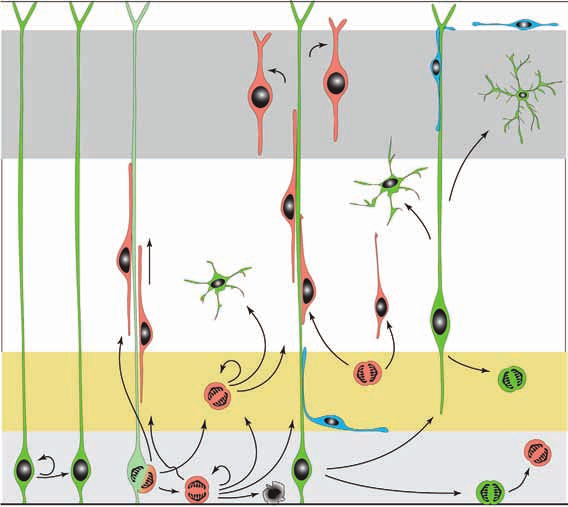
\includegraphics[width=0.8\textwidth]{rg_cells_division}\\
	\caption[A classical model of radial glial cells division processes \cite{Rakic2009}]{Illustration of a classical model of radial glial cells complex nonlinear division processes and neuronal migration \cite{Rakic2009}. From left to right: \acsp{npc} (green) originally divide symmetrically; During differentiation, \acsp{npc} become \acsp{rgc}, which divide asymmetrically, generating neurons or neural progenitor cells (orange). Neural progenitor cells eventually divide symmetrically into neurons. The majority of neurons in humans is produced by neuronal progenitors. A part of the generated neurons migrate radially towards the cortical plate, by attaching on the \acsp{rgc} projections; Eventually, after brain maturation, most \acsp{rgc} in humans undergo apoptosis (i.e. cell death) or generate neurons-supporting cells, such as astrocytes.}
	\label{fig:rgc}
\end{figure}


\subsection{The adult human cerebrum anatomic and functional properties}
 Human cerebrum is the center of sensations and thinking. The following excerpt provides a summarized anatomic \cite{Bear2016chapter7app} and functional \cite{Ferng2022} perspective.  As aforementioned, cerebrum is entirely produced  from the telencephalon during fetal development, with the telencephalic vesicles ending up becoming the two hemispheres, that remain connected through what is known as the \textbf{Corpus callosum}.  The side view of each hemisphere is named \textbf{lateral}, and the view of the inner side is called \textbf{medial}. The human cerebrum outer covering surface is called \textbf{cerebral cortex}, the region on which the current study focuses. The human cerebrum appears distinctly different from other organisms, mainly due to the \textbf{sulci} (i.e. grooves) and \textbf{gyri} (i.e. bumps), with them being the result of the tremendous expansion of the cerebral cortex surface area during fetal development, folding and wrinkling in order to fit the skull. The precise pattern of gyri and sulci varies significantly across populations, rendering the brain surface unique per individual. Under a biopsy dissection or a \ac{mri} scan, the cerebrum appears to consist of two distinctly colored types of matter, implying changes in composition and consistency; the gray matter, at the outer part of the cerebrum, which  contains the cell bodies, dendrites and the axon terminals, where all synapses are, and the white matter, at the inner part, made up of myelinated (i.e. biologically insulated) axons, which connect different parts of gray matter to each other (\autoref{fig:cerebissection}). Protective layers on top of the gray matter, called \textbf{meninges}, ensure that the brain does not come in contact with the outer bone, with the one attached on and marking the outer borders of the gray matter named \textbf{pial surface}. In this study, the midthickness surface is examined, a term referring to the surface halfway between the pial and white matter surface. 

\begin{figure}[H]
	\centering
	\begin{subfigure}{0.475\linewidth}
		
		\centering
		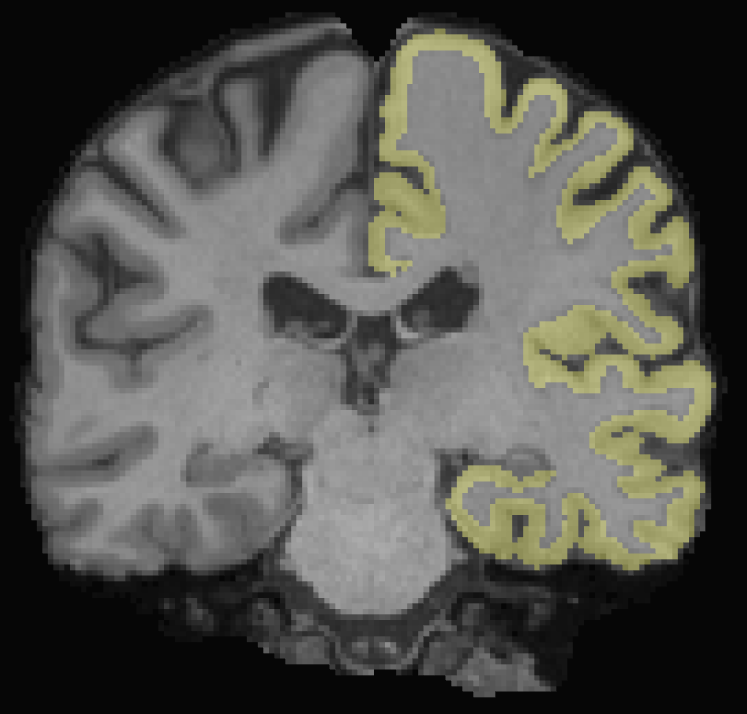
\includegraphics[width=0.475\linewidth]{coronal_section}
		\caption{Coronal section}
		\label{fig:coronal}
		
	\end{subfigure}
	\hfill
	\begin{subfigure}{0.475\linewidth}
		
		\centering
		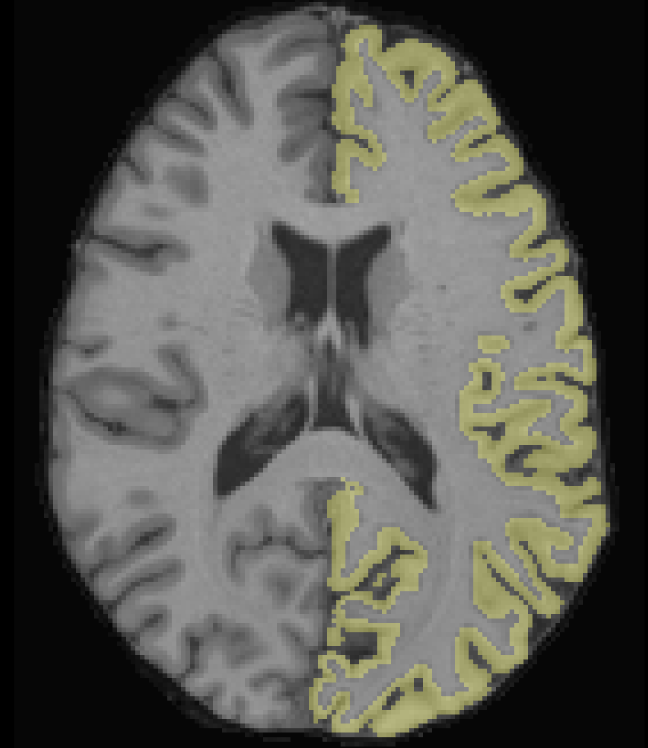
\includegraphics[width=0.475\linewidth]{axial_section}
		\caption{Axial section}
		\label{fig:axial}
	\end{subfigure}
	\vfill
	\begin{subfigure}{0.475\linewidth}
		
		\centering
		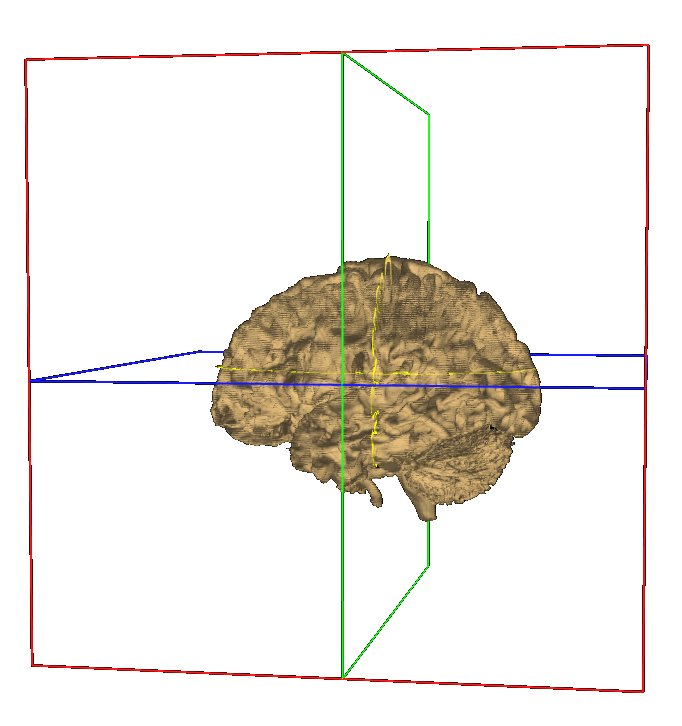
\includegraphics[width=0.475\linewidth]{3d_sections}
		\caption{\Ac{3d} sections map. Green rectangle corresponds to the coronal section plane (A) and
			blue rectangle to the axial section plane (B).}
	\end{subfigure}
	\caption[\Ac{mri} screening of gray and white matter]{Gray and white matter as seen from different sections, in an \ac{mri} screening, as retrieved from Freesurfer freeview routine. The gray matter is annotated with yellow color in the right hemisphere. Non brain regions have been removed.}
	\label{fig:cerebissection}
\end{figure}



\begin{figure}[H]
	\centering
	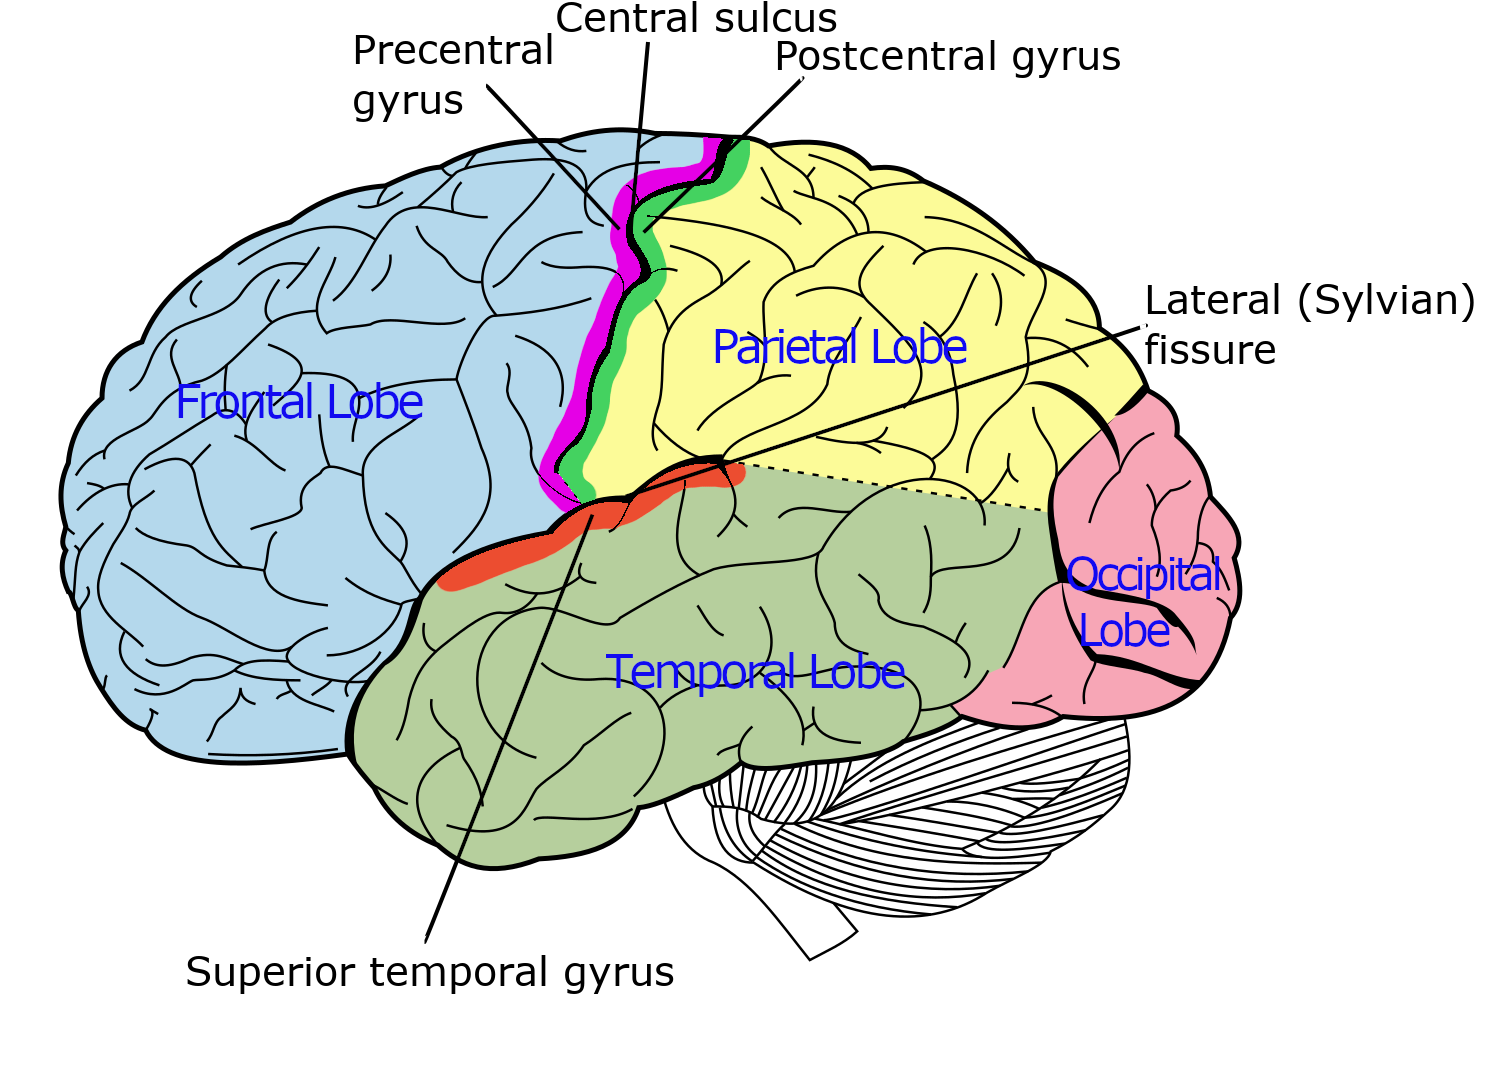
\includegraphics[width=0.8\textwidth]{1280px-Lobes_of_the_brain_NL.svg}
	\caption[A crude cerebrum partitioning]{Cerebrum lobes (blue font) and main gyri, sulci and fissures approximate positions (black font).}
	\label{fig:lobes}
\end{figure}

Efforts of partitioning the brain have been numerous throughout the years of medicine, with diverse resolution and purpose. Crudely, the cerebrum hemisphere is divided into lobes, that are named, by convention, after the bones of the skull that lie over them (\autoref{fig:lobes}).  A more detailed approach is based on the identification of the functional processes that take place in each part of the cortex, with Korbinian Brodmann being the first person constructing a 52-partitions experimentally based approximation of the hemisphere \cite{Brodmann1909} (\autoref{fig:corticalfunctions}). The main regions identified are:

\begin{figure}[H]
	\centering
	\begin{subfigure}{0.45\textwidth}
		\centering
		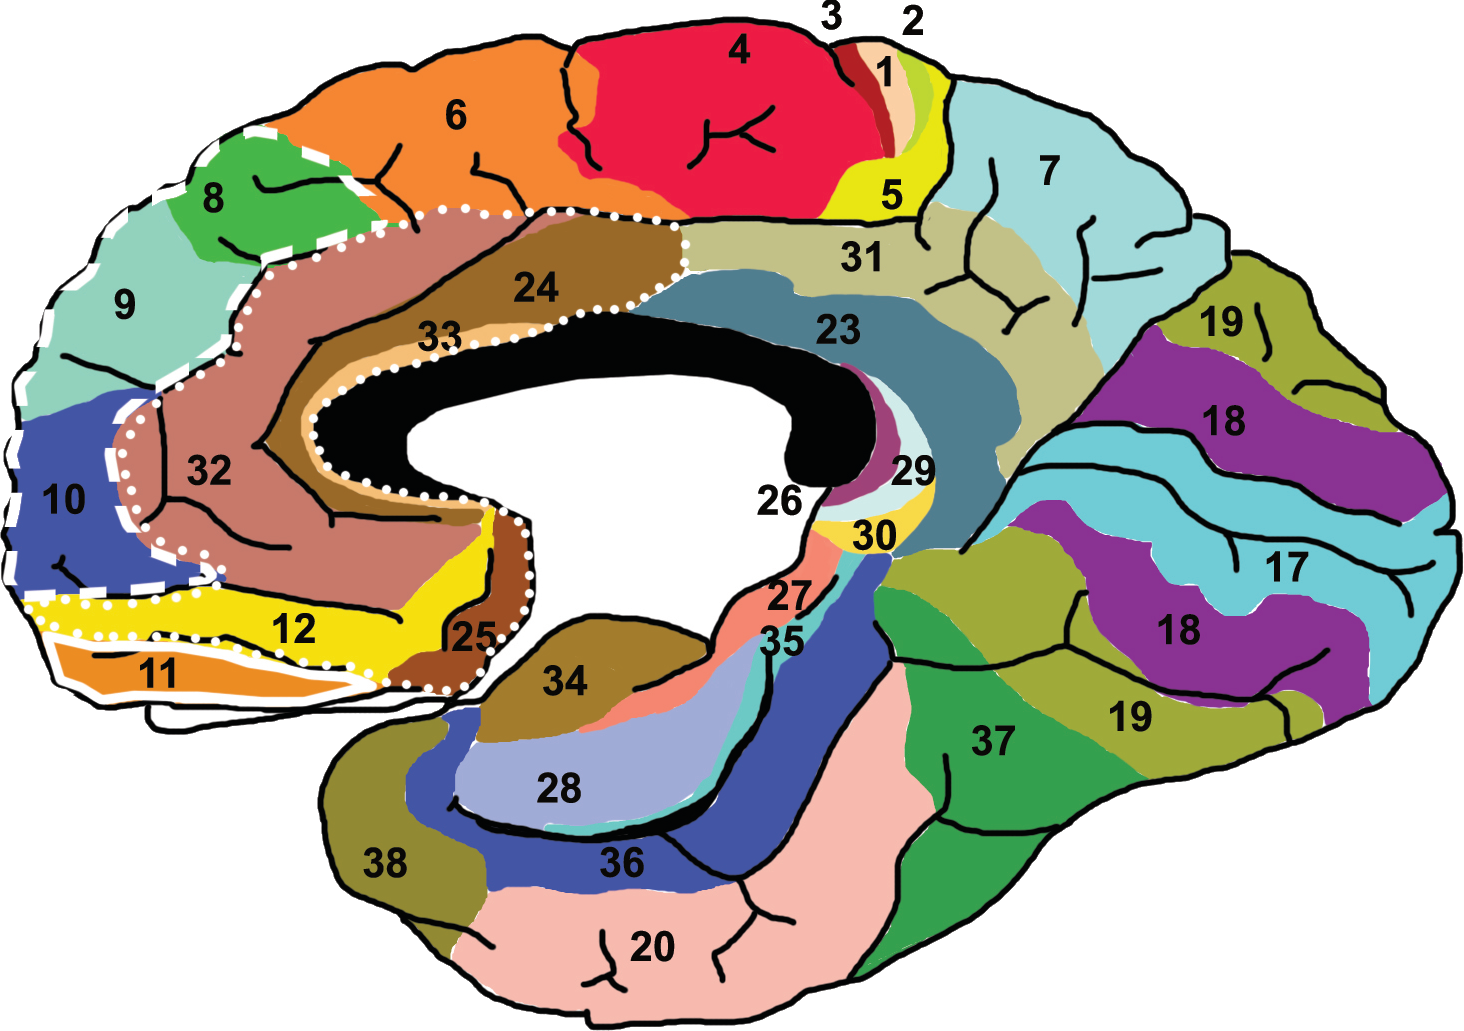
\includegraphics[width=\textwidth]{brodmann_medial}
		\caption{Medial surface}
		\label{fig:brodmann_medial}
	\end{subfigure}
	\hfill
	\begin{subfigure}{0.45\textwidth}
	\centering
	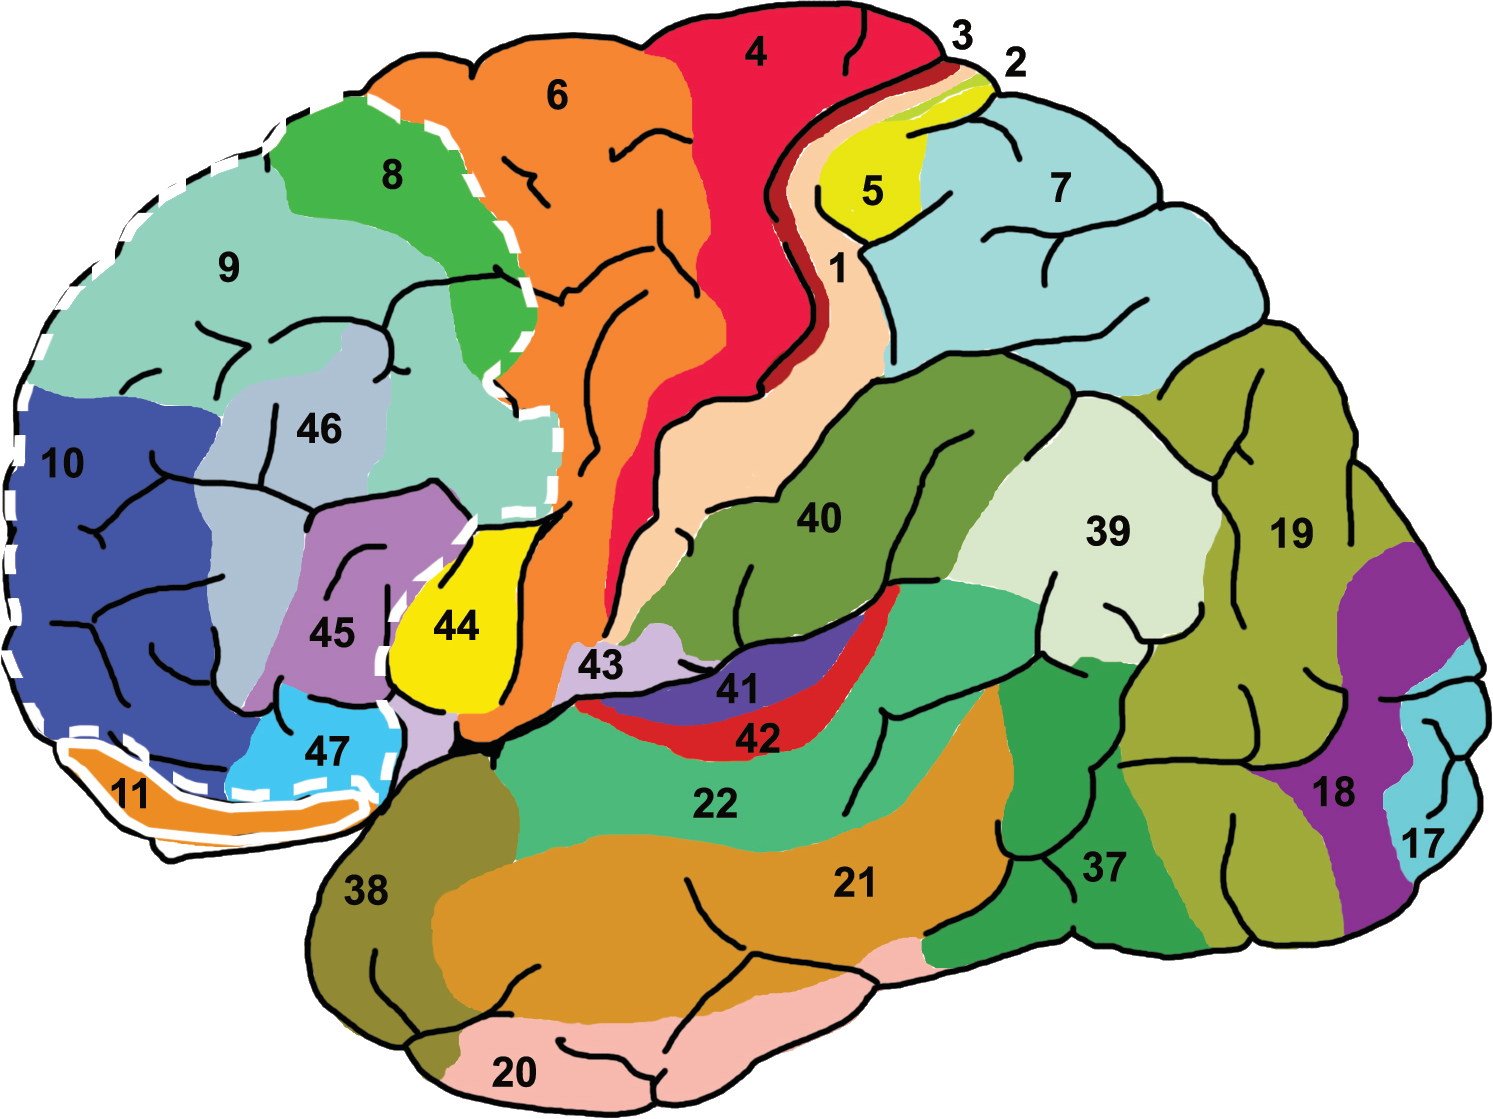
\includegraphics[width=\textwidth]{brodmann_lateral}
	\caption{Lateral surface}
	\label{fig:brodmann_lateral}
	
	\end{subfigure}
	\caption{Brodmann map of functional partitions.}
	\label{fig:corticalfunctions}
\end{figure}


\begin{itemize}

	\item{Sensory areas:
	\begin{itemize}
		\item {Somatosensory cortex (areas 1-3): the post-central gyrus (\autoref{fig:lobes}). It is responsible for the body-wide sensory information processing, such as touch, temperature and pain.}
		\item {Visual cortex (areas 17-19): occipital lobe surface. It constitutes the center of processing of visual information, as received from the optic nerve.}
		\item {Auditory cortex (areas 41,42): rostral posterior part of the temporal lobe. It processes auditory information, identifying fundamental sound characteristics, such as frequency and loudness.}
		\item {Gustatory cortex (area 43): An area behind the temporal lobe, responsible for taste signals processing.}
	\end{itemize}}

	\item{Motor areas, that are related to movement planning and manifestation:
	\begin{itemize}
		\item {Primary motor cortex (area 4): The precentral gyrus (\autoref{fig:lobes}). It is the center of voluntary movements execution, generating the electrical signals required for the neural impulses to be transmitted to the body muscles. }
		\item {Premotor cortex and supplementary motor area cortex (area 6): rostral part of the frontal lobe, anterior to the primary motor cortex. They are the center of motion planning and control, determining the sequence of movements required for a simple task to be performed.}
	\end{itemize}}
	\item{Association areas, which are related to perception, memory and thought processes:
	\begin{itemize}
		\item{Prefrontal cortex (areas 8-14,24,25,32,44-47): anterior part of the surface of the frontal lobe. It is centrally involved in cognitive control functions, spanning attention, salience detection, inhibitory control, working memory (i.e. short-term temporarily stored memory, related to a certain task), cognitive flexibility, empathy and pain processing \cite{Ong2019}. Areas 44 and 45, referred to as \textbf{Broca's region}, are responsible for speech production. Human prefrontal cortex remains one of the least functionally demystified parts of the cortex , presenting difficulties in every level of study, as it exhibits a higher relative size, higher cellular type variety, more complicated neuronal migration and denser connectivity patterns than other animals.\cite{Chini2021}}
		\item {Inferior temporal cortex (areas 20,21): caudal part of the temporal lobe cortex. It is responsible for the aggregation of the processed visual information towards a meaningful interpretation, supporting object recognition.}
		\item {Posterior parietal cortex (areas 5,7): posterior part of the parietal lobe surface. It processes sensory information produced from  all six senses to construct a semantic representation of the person's surroundings, leading to motion planning and spatial reasoning.}
		\item{Cingulate gyrus (areas 23-24,28,33): an arch-like fold rostrally to corpus callosum. It is the conscious part of the \textbf{limbic system}, which is the center of emotions, instinct and reflex responses.}
	\end{itemize}
}	
\end{itemize}

 Recently, with the advance of imaging methods, maps have been manufactured, to automatically partition the \ac{mri} extracted \ac{3d} cortical surface, based on morphological characteristics. One such gyral-based atlas, \ac{dk}, is derived from the changes in curvature under an expert-driven model of gyri locations \cite{Desikan2006} and provides automatic \textbf{cortical parcellation}, aligned to the Brodmann functional partitioning (\autoref{fig:dk}). This atlas is going to be used throughout the proceeding analysis for the quality control of applied segmentation techniques.
 
 \begin{figure}[H]
 	\centering
 	\includesvg[width=0.8\textwidth]{dk_left}\\
 	\caption[Desikan-Killiany atlas on midthickness surface]{\Acl{dk} atlas, mapped on the midthickness surface of the left hemisphere, with the medial (left) and the lateral (right) views displayed.\cite{Dickie2019} Different colors represent different partitions. The black region has not been mapped.}
 	\label{fig:dk}
 \end{figure}
 
 
 
\subsection{Reported general human cortex symmetry traits}
Although human cortex exhibits roughly symmetric structure, the symmetry is systematically suppressed, not only due to the environment, with plasticity playing central role, but also because of genetic factors, as explained in the previous sections. An asymmetric pattern is manifested across adult individuals, irrelevantly of their upbringing, comprising, therefore, a characteristic of the human species, while general abnormalities in this pattern are related to the occurrence of mental disorders, such as autism or developmental language disorder \cite{Herbert2005}\cite{Kong2022}. Some of the most prominent asymmetric traits across healthy individuals are the following:
\begin{itemize}
	\item{Yakovlevian torque (\autoref{fig:yaktorque}): the right hemisphere prefrontal lobe and the left hemisphere occipital lobe tend to cross the midsagittal plane, extending towards the other hemisphere \cite{Kuo2022}. This creates a phenomenon of counter-clockwise warping, making the whole brain appear slightly leftwards rotated, while also making an impression on the inner part of the skull, called \textbf{petalia}. Increased left hemisphere occipital lobe extension, possibly caused by enlarged left lateral ventricle, is correlated with bipolar disorder\cite{Maller2015}. Rising absence of the torque during aging is connected to schizophrenia  and other mental disorders \cite{Ribolsi2014}.}
	\item{Peri-Sylvian asymmetry: the left Sylvian (lateral) fissure is longer and sharper than the right one, while the right Sylvian fissure exhibits a more visible leftward curve, in the part where temporal lobe meets the parietal lobe, that is the auditory cortex, also called \textbf{planum temporale} \cite{Kuo2022}. The increased thickness of the right superior temporal lobe, that reduces the lateral fissure steepness, is attributed to increased white matter volume. Such trait has been reported to be gender-related, with males exhibiting greater asymmetry than females, as noted in previous studies, with steroid hormone receptor activity and steroid metabolic process related genes \cite{Guadalupe2015}.}
	\item{Central sulcus asymmetry: the right hemisphere central sulcus is deeper and larger \cite{Kuo2022}. Larger asymmetry appears to be correlated with \ac{adhd} \cite{Li2015}.}
	\item{Motor areas asymmetry: the motor areas are generally larger on the left hemisphere.}
\end{itemize}

Statistical modeling of the observed symmetry pattern can provide a hint on the significance  of genetic and environmental factors contribution\cite{Klingenberg2020}. The current study focuses on the genetic component, which has been diversely investigated across literature.


\begin{figure}
	\centering
%	\begin{subfigure}[t]{0.45\textwidth}
%		\centering
%		\includesvg[width=0.9\textwidth]{demoTorqueBrainAsymmetry/STAGE00DATA/averaged_torque_0_468}
%		\caption{Computed approximation of the Yakovlevian torque from working dataset, showing succinct clockwise rotation of 0.47 degrees (red line) versus the vertical black line.}
%		\label{fig:yakovlevian_computed}	
%	\end{subfigure}
%	\hfill
%	\begin{subfigure}[t]{0.45\textwidth}
\centering
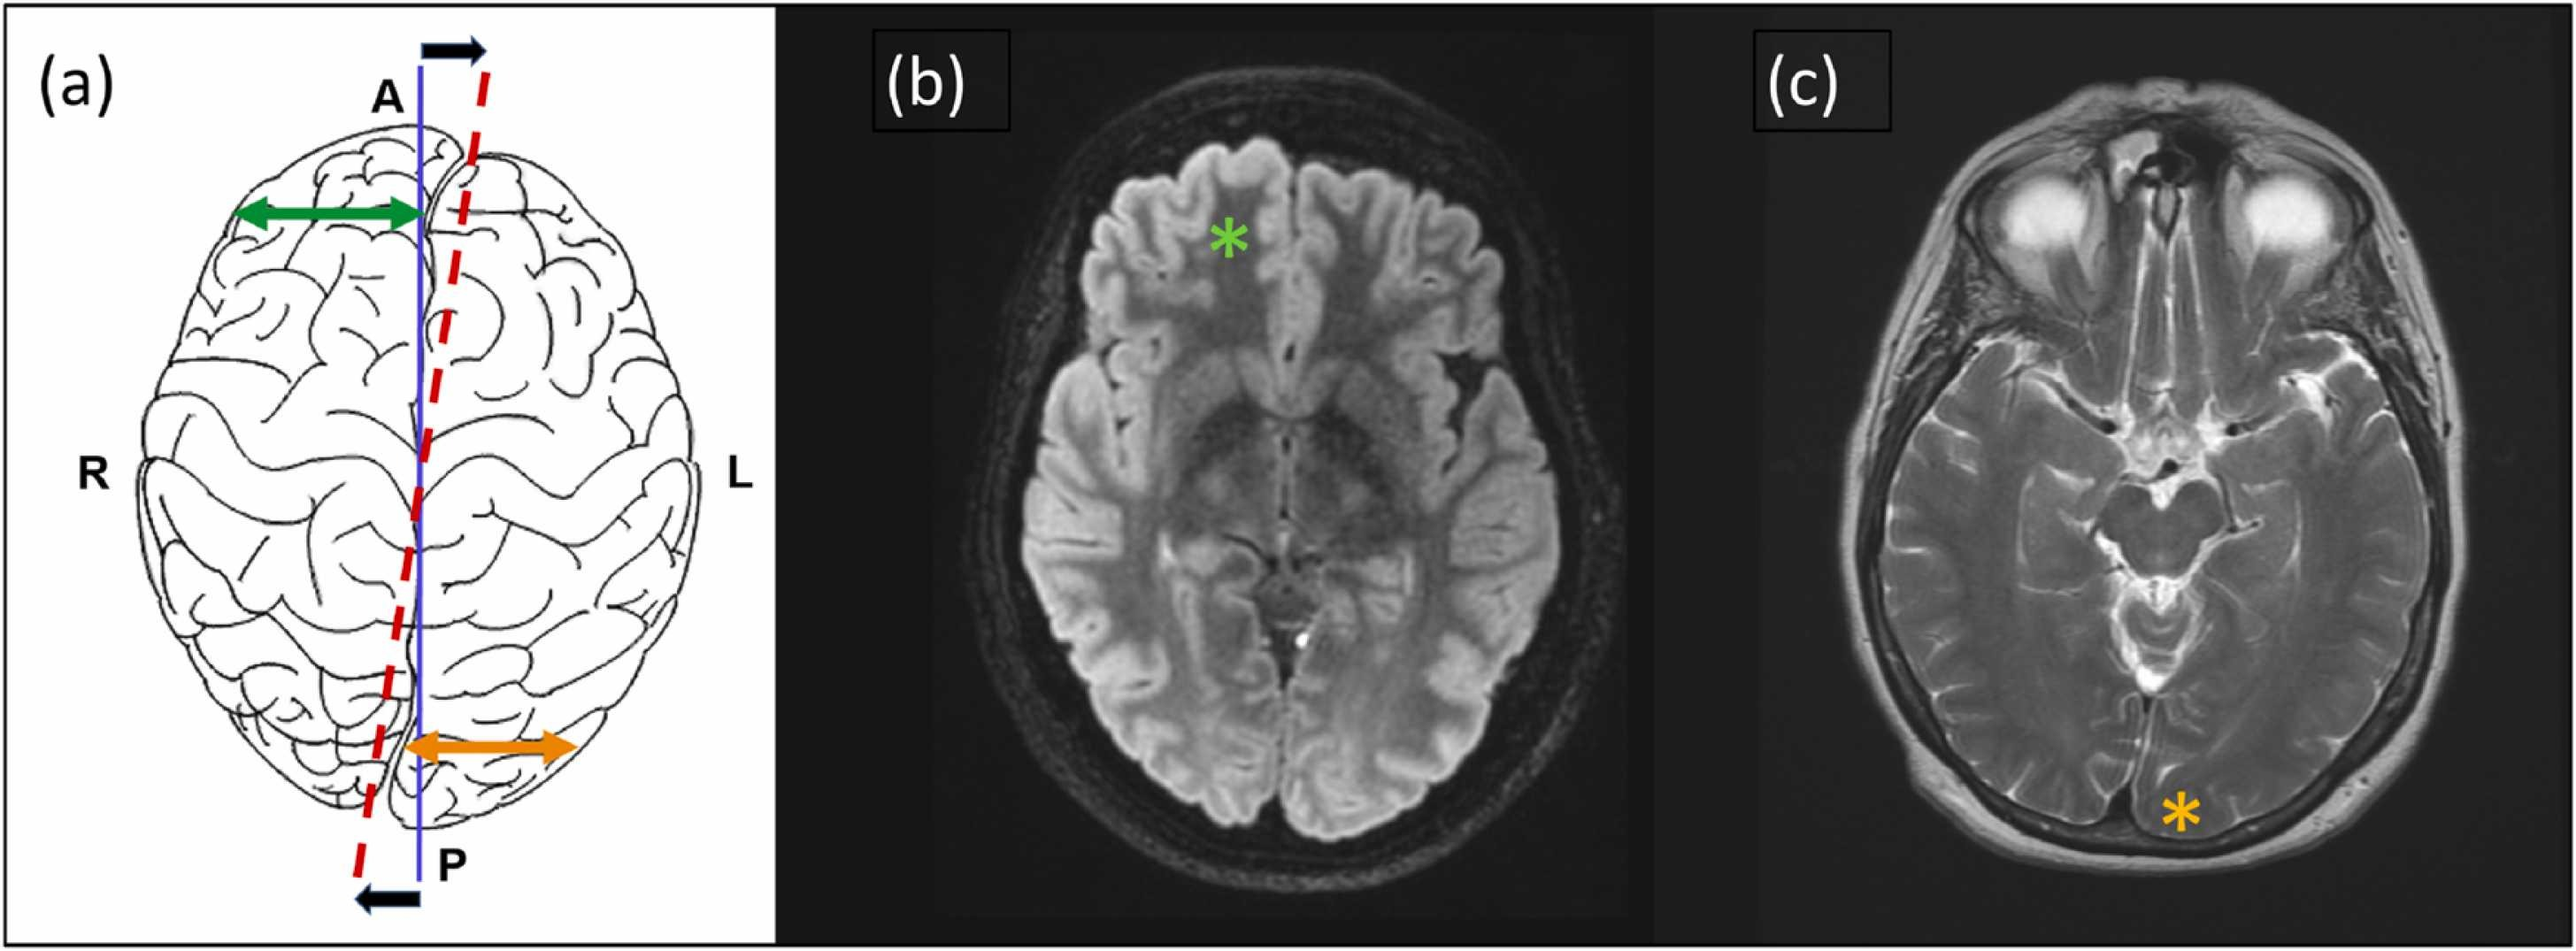
\includegraphics[width=\textwidth]{yakovlevian_external}
\caption[Yakovlevian Torque \cite{Kuo2022}]{Yakovlevian torque schematically illustrated (a), along with its manifestation in different axial sections for a single individual (b,c) \cite{Kuo2022}.}
%		\label{fig:yakovlevian_external}
%	\end{subfigure}
%\caption[Yakovlevian Torque \cite{Kuo2022}]{Illustration of the Yakovlevian torque. The angle of rotation in (A) was calculated by using the average angle of the longest edges, close to the midsagittal plane, of the convex hulls of the horizontal plane projection of each hemisphere midthickness surface, after shape normalization (see \autoref{subsec:shape_normalization}), per individual, across the studied population.}
\label{fig:yaktorque}
\end{figure}



\section{Genetics of multivariate quantitative traits}

\subsection{\Acf{mvgwas}}
\Ac{gwas} aim to relate genetic information, usually extracted from \acfp{snp} markers arrays, with a phenotypic trait. When the trait is dichotomous, measured as presence or absence of a certain quality, then \ac{gwas} are applied on a case-control fashion, where two cohorts, one exhibiting (case) the trait and another not (control), are compared. \cite{Uffelmann2021} In the present work, the focus is directed to quantitative traits, whose measurement takes continuous values.

\Acfp{snp} are characterized by single nucleotide base-pairs positions where two or more different alleles (i.e. variants of nucleotide bases) are observed, with the second most frequent allele appearing with a frequency, called \ac{maf}, higher than 1\%, a property that sets this term apart from the more general notion of a single-nucleotide variant. Being the most common type of polymorphism in the human genome, \acp{snp} were popularized on account of their considerable effect on influencing transcription. Apart from the direct case, where a \ac{snp} belongs to an exon and the alternate allele corresponds to a non-synonymous (the translated amino-acid differs) or a nonsense (the codon stops translation) mutation \cite{Ramensky2002}, the majority of registered \acp{snp} (88\%) reside in non-coding regions. They can have an impact on the physio-chemical properties and conformation of docking positions for \ac{dna}-binding enzymes, such as \acp{tf}, causing binding affinity changes, influencing transcription regulation and, ultimately, altering biological pathways relevant to dependent phenotypic traits \cite{Nishizaki2020}. As a matter of fact, 31\% of the known \ac{dna} elements, as reported by the ENCODE project, the human genome encyclopedia, appear to be part of \acp{tf} binding domains \cite{Dunham2012}.

Phenotypic differences among individuals, described by the trait variance $V_p$,  are the result of genetic variation $V_g$, known as \textbf{heritability}, environmentally induced variation $V_e$ and developmental noise $V_d$ (the deviations observed when environment and genetics are controlled), formally denoted as $V_p=V_g+V_e+V_d$ \cite{Vogt2020}. The genetic information content $V_g$ is \textit{approximated} by the amount of variation the alleles occurrence of a certain subset of \acp{snp} translated to variation in the studied trait properties.  The presence of a minor allele signifies divergence from the general population characteristics, and hence implies that information is contained in that \ac{snp}.  The relationship of each \ac{snp} with the phenotypic trait is statistically represented by a certain genetic model. Under the assumption of an \textbf{additive model}, if a certain minor allele occurs in both \ac{dna} strands, i.e the allele is homozygous at that locus, then its effect is double compared to the heterozygous case, independently of which strand is carrying it. This hypothesis requires no prior knowledge and makes no further assumptions regarding the alleles dynamics, that is the degree of dominance of each allelic variant. The described model, for a single quantitative trait (dependent variable) and a \ac{snp} with a single minor allele (assumed independent variable) can be formulated using a univariate linear regression $y = \beta x$, with $y$, ranging from 0 to 2, being the number of the allelic occurrences, $x$ being the phenotypic trait and $\beta$ the \ac{snp} effect. A \ac{snp} is then considered to have significant effect on the trait, if its calculated effect and the effective population size contradicts the null hypothesis $H_0$ of no association given an arbitrary probability cutoff \cite{AlejandroGonzalez-Chica2015}. Low sample size affects the type I error of the detection, namely the presence of false negatives that confirm the alternate hypothesis. $H_0$ is represented by a $\chi^2$ distribution with 1 \ac{dof}. The probability threshold is derived based on an empirical value, fixed to 0.05, corrected using the Bonferroni correction for multiple independent tests, hence $\frac{0.05}{N_t}$ with $N_t$ the number of \acp{snp}. The method is rather conservative, therefore usually cutoffs are computed by replacing the number of tests with the amount of independent common \acp{snp} for a given population. Based on the findings of the International Hapmap Project, this amounts approximately between 200,000 to 1 million \textbf{tag} \acp{snp}, i.e. \acp{snp} that are representative in high \ac{ld} regions, where non-random association of genetic loci is prevalent \cite{Belmont2003}. Therefore, the cutoff threshold $5\times 10 ^ {-8}$ is used. The p-values are most commonly converted to values proportional to significance, by applying the $-\log_{10}{p}$ transformation.   The \ac{ld} phenomenon, often locally observable, causes seemingly continuous p-value spikes to appear when plotting the data points, with the lead, or functional, \ac{snp}, the one with the greatest local significance (i.e. the lowest locally recorded p-value), being `supported` by lesser significant \ac{snp} in its surroundings, producing as a result a scatter plot, with \acp{snp} $-\log_{10}{p}$ values uniformly placed on x axis (i.e. ignoring their actual positions in the genome), that resembles the Manhattan city landscape (\autoref{fig:gwas_example}).

 \begin{figure}[H]
 	\begin{subfigure}[t]{0.45\textwidth}
	\centering
	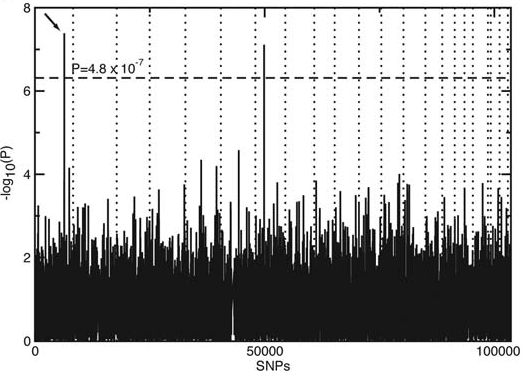
\includegraphics[width=0.9\textwidth]{gwas_2005}
	\caption{}
	\label{fig:gwas_2005}
	\end{subfigure}
	\hfill
	\begin{subfigure}[t]{0.6\textwidth}
		\centering
		\includesvg[width=0.9\textwidth]{asymmetry/genomeDemo/STAGE00DATA/not_imputed/not_subsampled/gwas.svg}
		\caption{}
		\label{fig:gwas_example}
	\end{subfigure}
	\caption[Examples of \acs{gwas} Manhattan plots \cite{Klein2005}]{Examples of \ac{gwas}. In (A), the first recorded \ac{gwas} Manhattan plot \cite{Klein2005} is displayed, where the \ac{snp} in chromosome 1 (black arrow) with the most significant  effect, related to Complement H Factor Polymorphism, was identified to affect age-related macular degeneration disease propensity, one of the major causes of blindness among elderly. In (B), a \ac{gwas} scatter plot from the present work is shown, where the \acp{snp} spikes signal, attributed to \ac{ld}, is evident.}
\end{figure}



There are several design benefits and limitations of such a process. \ac{gwas} have been successful in revealing novel relationships between genes with known properties and a variety of observed phenotypic traits and clinical applications, presenting evidence of possible biological mechanisms related to genes with unknown function \cite{Tam2019}. They also empower population-specific comparative studies, at the level of how ethnicity or other kinds of population stratification affect a certain trait, while accommodating the possibility to investigate the effect of an allele no matter how frequently it might appear in the studied sample \cite{Tam2019}. On the other hand, it has been generally observed  that each \ac{snp} can only explain a small part of the heritability of a certain trait, with a large amount of the signal hidden in gene-to-gene interactions, that are not captured in this method, and possibly in \acp{snp} whose contribution has not been considered significant enough. To remedy the latter issue, larger sample size is ideally required. TO BE CONTINUED/FIXED



However, the analyzed phenotype is described by more than one properties, that are related to the different landmarks composing the cortex of each individual. Also, a single \ac{snp} may exhibit more than one minor allele. The goal in this study, consequently, is to incorporate multi-allelic \acsp{snp} and, more importantly, multivariate phenotype, in a single hypothesis test per \ac{snp}, leading to what is called \ac{mvgwas}. In general, there is an abundance of strategies on how to perform \ac{mvgwas}, ranging from direct methods, that approximate the inputs relation either in an unbiased manner or making certain educated guesses, to more complex techniques, that increase statistical power by transforming the inputs, at the expense of explanatory ability \cite{Galesloot2014}. There are also methods that are based on the meta-analysis of outcomes from univariate studies, commonly used to juxtapose experiments from separate sources, for which the original data is missing, the experimental setup across studies is significantly different or a single study is computationally intractable \cite{Uffelmann2021,Cichonska2016}. Which approach performs best mainly lies on the dataset properties and the nature of the scientific question. Factors such as low sample size \cite{Sheng2021}, genes pleiotropic effects \cite{Fernandes2021} (i.e genes interacting through seemingly independent biological pathways) or within-study variability \cite{Usui2021,Jackson2011} tend to handicap the statistical modeling and increase the type I and II errors of the corresponding hypothesis tests. 





In this study, \ac{cca} was primarily chosen due to the high capacity in efficiently reducing the inputs dimensionality while preserving most information regarding their correlation. Diverse experiments, analyzed in \autoref{chap:gwas}, have been applied to identify the method that gives high fidelity results, consistent with relevant literature. The analysis outcome requires further processing, as explained in \autoref{sec:postprocessing}, to account for the main weakness of this method, that it does not consider the \ac{snp}-to-\ac{snp} effect, tackled using as proxy the notion of \ac{ld}, and subsequently to topologically and functionally enhance the filtered findings. Once this additional step has been performed, a cross-traits analysis is applied, described in \autoref{sec:metaanalysis}, where the \ac{da} genetic signature is compared with the signatures of phenotypic traits, analyzed in a similar study \cite{Naqvi2021}, the cerebral and facial shapes.





\section{Phenotypic trait analysis}\label{sec:phenotype_intro}
\subsection{Summary on cortex anatomy}
 
\subsection{Dataset Description}
 

The current study focuses on identifying the genetic landscape that composes the observed symmetry pattern, hence, subsequently, a brief introduction into how the genetic variations are being statistically modeled is provided.




\citet{Sha2021}


\subsection{Phenotypic partitioning}\label{sec:hsc}
\Acf{hsc} is an unsupervised method of iterative partitioning, that makes use of the distance matrix eigenvectors \cite{Ng2002}. It results into a binary tree structure (i.e. each parent shape is partitioned into two children). In the current study, a level-4 partitioning is performed, resulting into 31 partitions. Subsequently, they are transformed to the corresponding principal components that explain 80\% of the variance, for reasons of further dimensionality reduction. TO BE CONTINUED




\section{Breaking the complexity into parts}
TO BE EXPANDED

The present work evaluates the brain asymmetry genetic landscape in a coarse-to-fine segmentation, through the application of \ac{hsc}\cite{Ng2002}, discussed in \autoref{sec:hsc}. The technique has been used in a number of different related studies \cite{Claes2018}\cite{Naqvi2021}, yielding results that are in accordance with the underlying anatomic features. The main reason behind this partitioning is the intrinsic complexity of the studied phenotype, eliciting expected differences in the genomic profiles of each cerebral cortex region. The basic assumption made is that topologically close landmarks share similar genetic background. In general though, this type of distance-based clustering is governed by the least quantity of assumptions, regarding the shape or form of the cluster \cite{VonLuxburg2007}. The partitions' genetic juxtaposition is valuable for identifying which regions share similar significant genetic loci, highlighting the corresponding genes contribution, or showcasing the specialization of certain regions that share little to no similarities with their neighbors. Identifying the latter provides a way of mapping the developmental activation of each locus, bringing forth the opportunity to augment the results of related developmental studies \cite{Vijayakumar2016}.

\section{Searching for the origin}
TO BE EXPANDED

The genomic studies are performed under the framework of \ac{snp}-by-\ac{snp} \ac{cca}. 


\section{Data description}
In this study, targeted on humans, a cross section between the dependent cerebral asymmetry and the independent genetic factors is performed, in an effort to discover affiliated genetic regions and provide a novel understanding of the related genes cooperation. With the advent of technology capable to collect and process genomes from different individuals in relatively high speed, vast databases have been constructed. One of the main players in the data collection has been UK Biobank; a large-scale database from a randomized consortium of 500,000 individuals, whose genome has been collected, from whom  48,000 subjects had also participated in brain \ac{mri} collection process, as of December 2020 \cite{Littlejohns2020}. In this thesis, we exploit this newly acquired dataset to identify the key loci that are related to the human brain surface symmetry. Only healthy self-proclaimed white European individuals were considered. 

\section{Novelties based on related literature} 
 Due to the biological importance of cerebral bilateral asymmetry, it is a subject that has been rigorously studied from multiple viewpoints.
 \subsection{Evolution}
 From an evolutionary stand, it is extremely rare for the right conditions to occur, in order for any soft tissue specimen to be preserved, across a considerable amount of time. The only known way is through mineralization \cite{Purnell2018}. This fact renders a mammal's ancestor brain almost impossible to retrieve. Nevertheless, endocranial imprints have been used as a proxy to describe the relationships between hominids and their ancestors \cite{Balzeau2012}\cite{Neubauer2020}. The reason behind this phenotypic delegation is purely practical. The brain size and shape follow the container volume restrictions. Although such studies support the theory of propagating asymmetry among studied individuals, with the most evident signs of \ac{da} in human skulls, little information about the surface shape can be retrieved, as only the convex hull shape of the brain can be delineated from such process. Through the association of brain asymmetry with \acs{dna}, a universal code among organisms, it becomes possible to deploy tools used by evolutionary geneticists, to identify the phylogenetic tree of this complex trait, locating conserved regions among organisms and their predicted divergence in time, under a pleiotropic model \cite{Koch2021}.
 \subsection{Clinical studies}
 